%!TEX root = ../fbi.tex

\section{Construction of the featuresless boson insulator}

It was argued by Kimchi, et. al. \cite{kimchi2013} that this state represents a featureless Mott insulating phase of bosons on the honeycomb lattice.

\begin{equation}
\ket{\psi} = \prod\limits_{R} \sum\limits_{i \in R} b^{\dagger}_{i} \ket{0}
\label{eq:def}
\end{equation}


\subsection{PEPS Construction of honeycomb F.B.I.}
\begin{figure}[H]
	\centering
	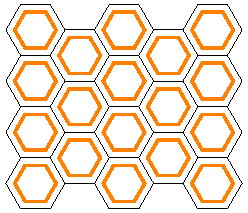
\includegraphics[width=0.6\columnwidth]{fbi3.pdf}
\end{figure}

\begin{figure}[H]
	\centering
	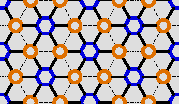
\includegraphics[width=0.6\columnwidth]{FI_PEPS2.pdf}
\end{figure}

\begin{figure}[H]
	\centering
	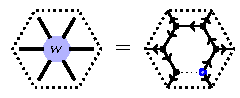
\includegraphics[width=0.6\columnwidth]{w_string.pdf}
\end{figure}

\begin{figure}[H]
	\centering
	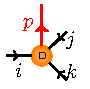
\includegraphics[width=0.3\columnwidth]{D_op.pdf}
\end{figure}
